% !TeX TS-program = txs:///duck
\documentclass{standalone}
\usepackage{tikzlings}
\usepackage{helvet}

\begin{document}

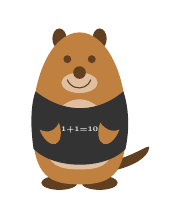
\begin{tikzpicture}
  \marmot
  
  \begin{scope}[xshift=-0.715cm]
    \fill[black!80!white] (0.1571,1.3606) .. controls (0.5321,1.0637) and (0.9558,1.0898) .. (1.2712,1.3606) .. controls (1.2712,1.3606) and (1.3905,1.0523) .. (1.2973,0.6266) .. controls (1.0335,0.3616) and (0.3947,0.3653) .. (0.1310,0.6303) .. controls (0.0564,1.1455) and (0.1571,1.3606) .. (0.1571,1.3606) -- cycle;
    \node[white,font=\tiny\bfseries,align=center,scale=0.5] at (0.715,0.87) {1+1=10};
    \fill[brown] (0.9784,0.9650) .. controls (0.9330,0.8404) and (0.9510,0.7194) .. (1.0185,0.6948) .. controls (1.0860,0.6703) and (1.1775,0.7514) .. (1.2229,0.8760) .. controls (1.0748,0.8115) and (0.9784,0.9650) .. (0.9784,0.9650) -- cycle (0.4123,0.6948) .. controls (0.4798,0.7194) and (0.4978,0.8404) .. (0.4524,0.9650) .. controls (0.4524,0.9650) and (0.3893,0.7888) .. (0.2079,0.8760) .. controls (0.2533,0.7514) and (0.3448,0.6703) .. (0.4123,0.6948) -- cycle;
  \end{scope}
  
\end{tikzpicture}

\end{document}